\section{Results}
\label{sec:results}

\begin{figure*}[t]
\begin{center}
\begin{tabular}{c@{\;}c@{\;}c@{\;}c@{\;}c@{\;}c@{\;}c@{\;}c@{\;}c@{\;}c}

\includegraphics[width=0.10\linewidth]{fig/supp/c07.png} &

\includegraphics[width=0.10\linewidth]{fig/supp/c07-sparse_dr.png} &

\includegraphics[width=0.10\linewidth]{fig/supp/c07-rgb2gray.png} &

\includegraphics[width=0.10\linewidth]{fig/supp/c07-ancuti2011.png} &

\includegraphics[width=0.10\linewidth]{fig/supp/c07-kim2009.png} &

\includegraphics[width=0.10\linewidth]{fig/supp/c07-smith2008.png} &

\includegraphics[width=0.10\linewidth]{fig/supp/c07-pr2006.png} &

\includegraphics[width=0.10\linewidth]{fig/supp/c07-gooch2005.png} &

\includegraphics[width=0.10\linewidth]{fig/supp/c07-rasche2005.png} \\

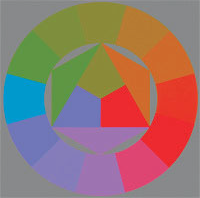
\includegraphics[width=0.10\linewidth]{fig/supp/c08.png} &
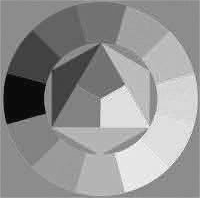
\includegraphics[width=0.10\linewidth]{fig/supp/c08-sparse_dr.png} &

\includegraphics[width=0.10\linewidth]{fig/supp/c08-rgb2gray.png} &
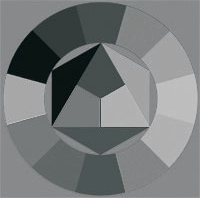
\includegraphics[width=0.10\linewidth]{fig/supp/c08-ancuti2011.png} &

\includegraphics[width=0.10\linewidth]{fig/supp/c08-kim2009.png} &

\includegraphics[width=0.10\linewidth]{fig/supp/c08-smith2008.png} &

\includegraphics[width=0.10\linewidth]{fig/supp/c08-pr2006.png} &

\includegraphics[width=0.10\linewidth]{fig/supp/c08-gooch2005.png} &
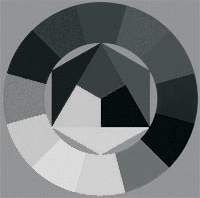
\includegraphics[width=0.10\linewidth]{fig/supp/c08-rasche2005.png} \\

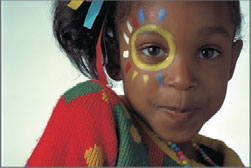
\includegraphics[width=0.10\linewidth]{fig/supp/c11.png} &
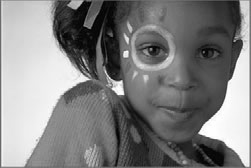
\includegraphics[width=0.10\linewidth]{fig/supp/c11-sparse_dr.png} &
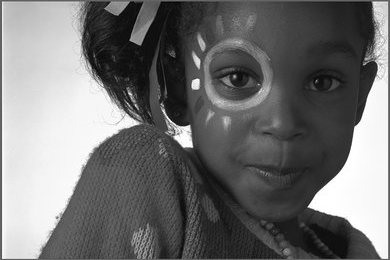
\includegraphics[width=0.10\linewidth]{fig/supp/c11-rgb2gray.png} &
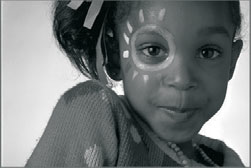
\includegraphics[width=0.10\linewidth]{fig/supp/c11-ancuti2011.png} &
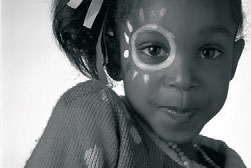
\includegraphics[width=0.10\linewidth]{fig/supp/c11-kim2009.png} &
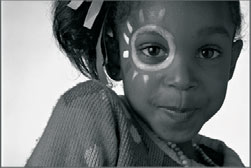
\includegraphics[width=0.10\linewidth]{fig/supp/c11-smith2008.png} &
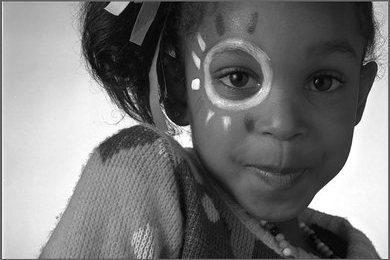
\includegraphics[width=0.10\linewidth]{fig/supp/c11-pr2006.png} &
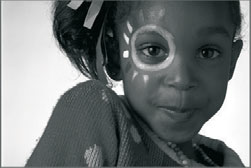
\includegraphics[width=0.10\linewidth]{fig/supp/c11-gooch2005.png} &
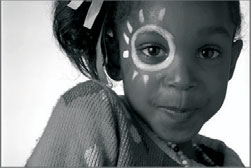
\includegraphics[width=0.10\linewidth]{fig/supp/c11-rasche2005.png} \\

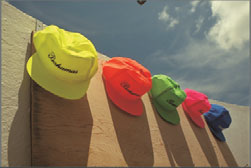
\includegraphics[width=0.10\linewidth]{fig/supp/c23.png} &
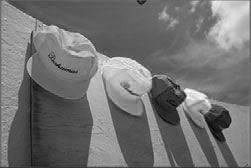
\includegraphics[width=0.10\linewidth]{fig/supp/c23-sparse_dr.png} &
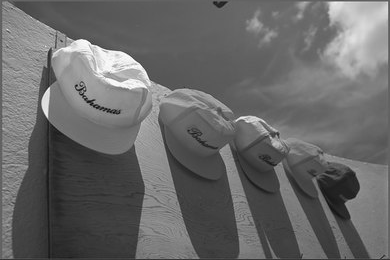
\includegraphics[width=0.10\linewidth]{fig/supp/c23-rgb2gray.png} &
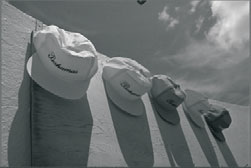
\includegraphics[width=0.10\linewidth]{fig/supp/c23-ancuti2011.png} &
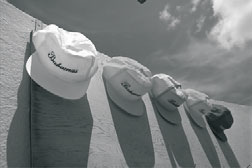
\includegraphics[width=0.10\linewidth]{fig/supp/c23-kim2009.png} &
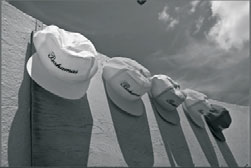
\includegraphics[width=0.10\linewidth]{fig/supp/c23-smith2008.png} &
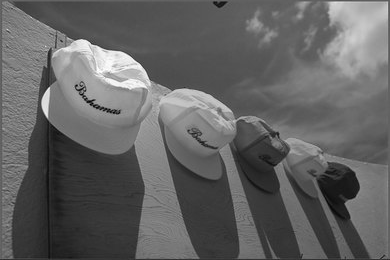
\includegraphics[width=0.10\linewidth]{fig/supp/c23-pr2006.png} &
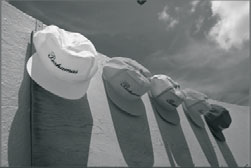
\includegraphics[width=0.10\linewidth]{fig/supp/c23-gooch2005.png} &
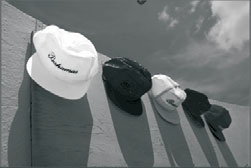
\includegraphics[width=0.10\linewidth]{fig/supp/c23-rasche2005.png} \\

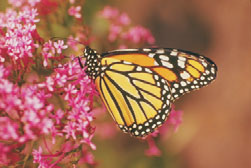
\includegraphics[width=0.10\linewidth]{fig/supp/c24.png} &
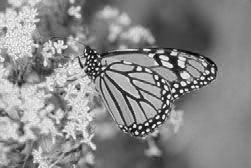
\includegraphics[width=0.10\linewidth]{fig/supp/c24-sparse_dr.png} &
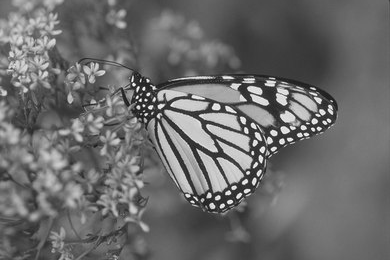
\includegraphics[width=0.10\linewidth]{fig/supp/c24-rgb2gray.png} &
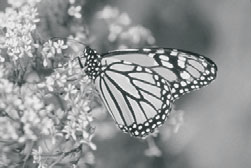
\includegraphics[width=0.10\linewidth]{fig/supp/c24-ancuti2011.png} &
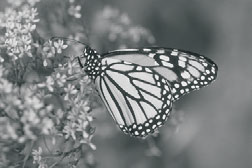
\includegraphics[width=0.10\linewidth]{fig/supp/c24-kim2009.png} &
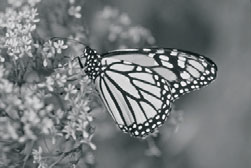
\includegraphics[width=0.10\linewidth]{fig/supp/c24-smith2008.png} &
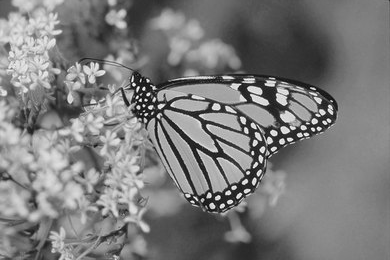
\includegraphics[width=0.10\linewidth]{fig/supp/c24-pr2006.png} &
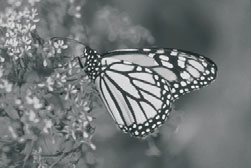
\includegraphics[width=0.10\linewidth]{fig/supp/c24-gooch2005.png} &
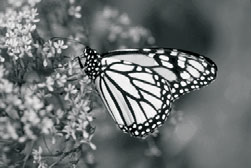
\includegraphics[width=0.10\linewidth]{fig/supp/c24-rasche2005.png} \\

color & ours & rgb2gray & Ancuti11 & Kim09 & Smith08 & \shortcite{Grundland:2007:DFC} & Gooch05 & Rasche05
\end{tabular}
\caption{
\textbf{Comparison with previous methods.}
From left to right: original color images, ours with default setting $\delta=20$ and $vw=0.1$,
standard rgb2gray in MatLab, Ancuti~\etal~\protect\shortcite{Ancuti:2011:ESG},
Kim~\etal~\protect\shortcite{Kim:2009:RCV}, 
Smith~\etal~\protect\shortcite{Smith:2008:AGA}, 
Grundland and Dodgson~\protect\shortcite{Grundland:2007:DFC}, 
Gooch~\etal~\protect\shortcite{Gooch:2005:CSC},
and Rasche~\etal~\protect\shortcite{Rasche:2005:RIG}.
From top to down: Three cases demonstrate that, comparing with previous methods, 
our algorithm maintain the visual appearance with
perceptually preserving the saliency, keeping the order in chromatics, and without
over enriching the contrast.
}
\label{fig:comparison}
\end{center}
\end{figure*}

We compare the results between our algorithm and previous decolorziation
methods~\cite{Ancuti:2011:ESG,Kim:2009:RCV,Smith:2008:AGA,Grundland:2007:DFC,Rasche:2005:DPR,Gooch:2005:CSC} in Figure~\ref{fig:comparison}.
With a suitable feature transform, we preserve contrast and saliency without suffering
from isoluminants in the input image.
As a global color mapping, our algorithm avoid to create artifacts such as halos, noise
or broken segments in pixel-based 
computation~\cite{Bala:2004:SCT,Gooch:2005:CSC,Rasche:2005:RIG}.
In contrast with other global methods, we straightly preserve the most salient region
in the images to exploit the power of linear operator as the demonstration in
Figure~\ref{fig:saliency}.
Comparing with the most recent work by Ancuti~\etal~\cite{Ancuti:2011:ESG},
both of our works focusing on saliency preserving transformation,
our method further avoid to map different chromatics into the same luminance
and boost the contrast more as the demonstration in Figure~\ref{fig:comparison}.

\subsection{Contrast enhancement imaging}

\begin{figure*}[t]
\begin{center}
\begin{tabular}{ccccc}
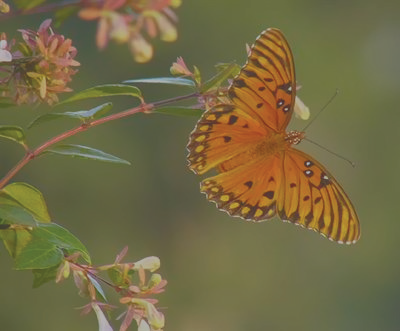
\includegraphics[width=0.18\linewidth]{fig/i02.png} &
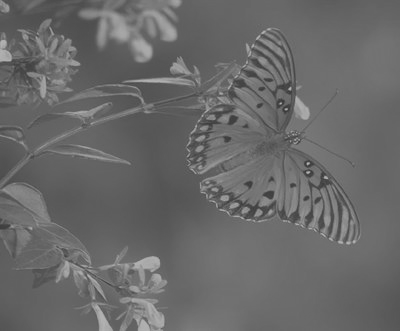
\includegraphics[width=0.18\linewidth]{fig/i02-rgb2gray.png} &
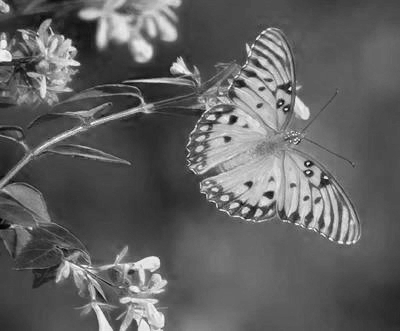
\includegraphics[width=0.18\linewidth]{fig/i02-sparse_dr.png} &
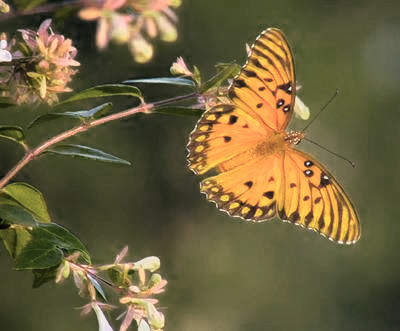
\includegraphics[width=0.18\linewidth]{fig/i02-enhance.png} &
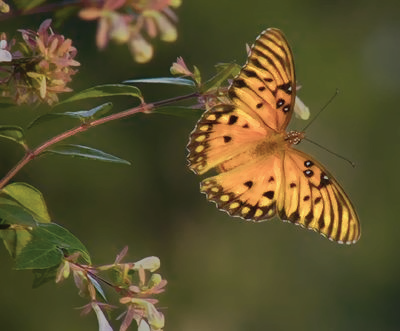
\includegraphics[width=0.18\linewidth]{fig/i02-iccp2012.png} \\
\includegraphics[width=0.18\linewidth]{fig/i04.png} &
\includegraphics[width=0.18\linewidth]{fig/i04-rgb2gray.png} &
\includegraphics[width=0.18\linewidth]{fig/i04-sparse_dr.png} &
\includegraphics[width=0.18\linewidth]{fig/i04-enhance.png} &
\includegraphics[width=0.18\linewidth]{fig/i04-iccp2012.png} \\
color & rgb2gray & ours & ours+color & Lu12
%
\end{tabular}
\caption{
\textbf{Salient region enhancement.}
From left to right: original color image, rgb2gray, our grayscale image, our enhancing
image, Lu~\etal's image~\protect\cite{Lu:2012:CPD}.
Our graysacle image with enhancing contrast can use to boost the contrast and
relight the region of interest.
}
\label{fig:enhancing}
\end{center}
\end{figure*}

\begin{figure*}[t]
\begin{center}
\begin{tabular}{cccc}
\includegraphics[width=0.2\linewidth]{fig/r08.png} &
\includegraphics[width=0.2\linewidth]{fig/r08-rgb2gray.png} &
\includegraphics[width=0.2\linewidth]{fig/r08-sparse_dr.png} &
\includegraphics[width=0.2\linewidth]{fig/r08-enhance.png} \\
color & rgb2gray & ours & ours+color
%
\end{tabular}
\caption{
\textbf{Image detail enhancement.}
Our grayscale image makes original image sharpen.
}
\label{fig:dehazing}
\end{center}
\end{figure*}

To enrich the contrast of the original image, we substitute the {\it L} of {\it L*a*b}
by our salient-enhancing monochrome image. Comparing with Ju~\etal~\cite{Lu:2012:CPD},
our method prefers to map high salient region into bright luminance. 
Therefore, the enhancing image not only increase the contrast but also 
light up the particular region of interest as showing in Figure~\ref{fig:enhancing}.

The enhancing contrast image can help to dehaze with the same strategy. 
Figure~\ref{fig:dehazing} demonstrates the dehazed imaging obtained by our method.

% weakness of our method
\ignore{
\begin{figure}[t]
\begin{center}
\begin{tabular}{cccc}
\includegraphics[width=0.2\linewidth]{fig/collect.jpg} &
\includegraphics[width=0.2\linewidth]{fig/collect-sortseg.png} &
\includegraphics[width=0.2\linewidth]{fig/collect-sparse_dr.png} &
\includegraphics[width=0.2\linewidth]{fig/collect-rgb2gray.png} \\
color & importance map & ours & rgb2gray
%
\end{tabular}
\caption{
\textbf{Situation with multiple salient subjects.}
Our framework compute the importance of superpixels as the hint of decolorization.
As second column present, more lighter the map is, more salient of that region.
The result distinguishes the color between the flower and background, but ignore
other subjects which might be more significant in other viewers observation.
}
\label{fig:collect}
\end{center}
\end{figure}
%
\begin{figure}[t]
\begin{center}
\begin{tabular}{cccc}
\includegraphics[width=0.2\linewidth]{fig/c04.png} &
\includegraphics[width=0.2\linewidth]{fig/c04-seg.png} &
\includegraphics[width=0.2\linewidth]{fig/c04-sparse_dr.png} &
\includegraphics[width=0.2\linewidth]{fig/c04-rgb2gray.png} \\
color & segmentation & ours & rgb2gray
%
\end{tabular}
\caption{
\textbf{Situation with failure of segmentation.}
Using default parameters suggested in~\protect\cite{Felzenszwalb:2004:EGI},
the segmentation has a flaw in the boundary between the purple ball and the table.
It makes an incorrect codeword due to the color distortion from purple to imperial blue.
}
\label{fig:segmentation}
\end{center}
\end{figure}
%
Our framework relies on saliency map and region segmentation.
This dependency limits our framework in some cases.
First, since we only focus on the most salient subject in the image, 
our algorithm fail to handle the images with multiple salient region.
The problem may cause by noises which effected the salient estimation.
For example, specular reflection or the stain on the camera lens may form
an unwanted segments.
Alternate the detectors, such as Itti~\etal's~\cite{Itti:1998:AMS} and 
Hou~\etal's~\cite{Hou:2012:ISH}, might help for generating different
salient distribution.
However, salient region specific to different people, and there were no
existed methods have completed solved this problem.
Figure~\ref{fig:collect} shows that there are various subjects in the input canvas.
Second, failure segmentation would distort the codewords of dictionary.
It would effect the decolorization because the optimization in (\ref{eqn:optimization})
is not going to process for the actual distribution of the input image.
Figure~\ref{fig:segmentation} shows this case.
}
